\documentclass[conference]{IEEEtran}
\IEEEoverridecommandlockouts
\usepackage{cite}
\usepackage{listings}
\lstdefinestyle{ieee}{
  basicstyle=\ttfamily\footnotesize,
  numbers=none,
  breaklines=true,
  breakatwhitespace=true,
  columns=fullflexible,
  keepspaces=true,
  frame=tb,
  aboveskip=6pt,
  belowskip=6pt,
  xleftmargin=0pt
}
\lstset{style=ieee}
\usepackage{amsmath,amssymb,amsfonts}
\usepackage{algorithmic}
\usepackage{graphicx}
\usepackage{textcomp}
\usepackage{xcolor}
\usepackage{url}
\usepackage{verbatim}
\usepackage{booktabs}
\usepackage{tabularx}
\usepackage{makecell}
\usepackage{siunitx}
\usepackage{threeparttable}
\sisetup{detect-all}
\newcolumntype{Y}{>{\centering\arraybackslash}X}

\def\BibTeX{{\rm B\kern-.05em{\sc i\kern-.025em b}\kern-.08em
    T\kern-.1667em\lower.7ex\hbox{E}\kern-.125emX}}

\begin{document}

\title{eBPF SYN Flood Firewall: Integrated XDP and SYNPROXY Defense\\}

\author{
\IEEEauthorblockN{Alessandro Martini, Andrea Piroddi, Roberto Girau,
Giovanni Pau, Franco Callegati, Andrea Melis}
\IEEEauthorblockA{
Department of Computer Science and Engineering\\
University of Bologna, Cesena, Italy\\
Emails: \{andrea.piroddi, roberto.girau, giovanni.pau,
franco.callegati, a.melis\}@unibo.it\\
Alessandro Martini: alessandro.martini10@studio.unibo.it
}
}

\maketitle

% ─────────────────────────────────────────────────────────────────────────────
\begin{abstract}
Denial-of-Service (DoS) and Distributed Denial-of-Service (DDoS) attacks,
particularly SYN floods, continue to threaten the availability of networked
services.
This paper investigates the integration of XDP-based early packet filtering
with SYNPROXY-based TCP validation within a unified in-kernel firewall
architecture.
By leveraging eBPF programs in the eXpress Data Path (XDP), the proposed
approach performs lightweight filtering at the earliest stage of packet
processing, while SYNPROXY ensures correct connection establishment through
SYN cookie validation.

We evaluate three configurations---XDP-only, iptables (SYNPROXY)-only, and
a combined XDP+SYNPROXY approach---under single-source, distributed, and
spoofed SYN flood attacks, on both a physical testbed and a scalable
emulated environment based on Mininet with statistical validation
(3~independent runs, $N=120$ measurements per run).

The results show that the effectiveness of each defense mechanism strongly
depends on the attack model.
Under single-source attacks, XDP-only reduces CPU utilization by $35$\%
compared to iptables+SYNPROXY ($43.8$\% vs.\ $69.9$\%) while maintaining
identical service availability.
Under distributed attacks, XDP+SYNPROXY achieves the lowest latency
($0.038 \pm 0.039$\,s) and CPU ($58.3 \pm 0.8$\%), outperforming all
other configurations.
Under spoofed attacks, iptables+SYNPROXY achieves the lowest latency
($0.049 \pm 0.022$\,s), confirming the value of connection-level validation
against high-entropy traffic.
On physical hardware, the combined architecture achieves up to $98.6$\%
service success rate under spoofed attacks.
A threshold sensitivity analysis ($\tau \in \{50,100,200,500\}$~SYN/IP
per 2\,s) identifies $\tau=200$ as the optimal operating point for the
combined configuration.

These findings demonstrate that no single mitigation strategy is
universally optimal.
Combining stateless and stateful mechanisms enables adaptive defense
strategies that balance performance and robustness depending on attack
characteristics.
\end{abstract}

\begin{IEEEkeywords}
eBPF, iptables, XDP, DDoS, SYN flood, firewall, SYNPROXY, conntrack,
Mininet
\end{IEEEkeywords}

% ─────────────────────────────────────────────────────────────────────────────
\section{Introduction}

In recent years, the extended Berkeley Packet Filter (eBPF) has emerged as
a powerful mechanism for executing sandboxed programs within the Linux
kernel, enabling flexible and high-performance network traffic
processing~\cite{ebpf}.
Building on eBPF, the eXpress Data Path (XDP) provides a fast in-kernel
dataplane that allows packets to be processed at the earliest point in the
networking stack, directly at the network interface driver
level~\cite{HighPerfXDP}.

Figure~\ref{fig:ebpf_probe} illustrates the architecture of an XDP-based
filtering framework.
Incoming packets are intercepted before entering the kernel networking
stack, allowing eBPF programs to apply filtering logic with minimal latency.
This early processing enables operations such as packet dropping or rate
limiting to be performed before costly mechanisms like connection tracking
or socket allocation, thereby reducing CPU load and improving resilience
under high traffic conditions.

Denial-of-Service (DoS) and Distributed Denial-of-Service (DDoS) attacks,
particularly TCP SYN floods, remain a major threat to network
availability~\cite{TahirPaper}.
These attacks exploit the TCP three-way handshake to exhaust server
resources, often leveraging large-scale botnets or spoofed source addresses.
Traditional defenses, such as iptables-based firewalls, struggle to handle
the scale and dynamics of modern attacks~\cite{applsci13}.
As a result, programmable and high-performance in-kernel defenses have
become increasingly important.

XDP-based filtering enables high-rate packet dropping and efficient
mitigation of volumetric attacks.
However, most existing XDP-based solutions rely primarily on stateless
filtering mechanisms (e.g., per-source rate
limiting)~\cite{HighPerfXDP}, which can be ineffective against spoofed
attacks where source IP addresses change rapidly.
Conversely, stateful approaches such as SYNPROXY provide robust connection
validation using SYN cookies, but introduce additional processing overhead.

Recent work has explored combining XDP with SYNPROXY to improve
performance~\cite{NVidiaSynFlood}.
However, the trade-offs between stateless filtering and stateful validation
under different attack scenarios remain insufficiently understood, and
existing evaluations lack statistical rigor and reproducibility.

In this paper, we investigate the integration of XDP-based early filtering
with SYNPROXY-based validation within a unified in-kernel architecture.
Rather than assuming a universally optimal solution, we focus on
understanding how different mechanisms behave under varying attack models,
including single-source, distributed, and spoofed SYN floods.
To improve reproducibility and statistical validity, we complement the
physical testbed with a Mininet-based emulated environment, performing three
independent runs of 60\,s each (yielding $N=120$ measurements per
configuration) and reporting mean and standard deviation for all metrics.

\subsection*{Contributions}

This paper makes the following contributions:

\begin{itemize}
  \item We design and implement a layered in-kernel defense combining
        XDP-based early filtering with SYNPROXY-based TCP validation,
        with a runtime-configurable rate limiting threshold exposed via
        a BPF map.
  \item We provide a statistically rigorous experimental comparison
        (3~independent runs, $N=120$ per run) of XDP-only,
        iptables+SYNPROXY, and combined XDP+SYNPROXY configurations under
        multiple attack models, on both physical and emulated testbeds.
  \item We introduce a scalable Mininet-based evaluation environment with
        Open vSwitch that enables systematic, reproducible testing across
        varying attacker counts and traffic rates.
  \item We characterize a previously unreported behavior: under spoofed
        attacks, iptables+SYNPROXY achieves \emph{lower} latency than
        XDP-only ($0.049$\,s vs.\ $0.143$\,s), revealing that
        connection-level validation provides a latency advantage when
        stateless filtering is ineffective.
  \item We perform a systematic threshold sensitivity analysis
        ($\tau \in \{50,100,200,500\}$~SYN/IP per 2\,s window) and
        identify $\tau=200$ as the optimal operating point for the
        combined XDP+SYNPROXY configuration, minimizing latency under
        spoofed attacks while avoiding false positive-induced
        retransmissions.
  \item We analyze performance trade-offs between latency, CPU
        utilization, and service success rate, and quantify practical
        significance using Cohen's $d$ effect size, providing principled
        guidance for real-world deployment.
\end{itemize}

The remainder of this paper is organized as follows.
Section~\ref{sec:related} reviews related work.
Section~\ref{sec:systemdesign} presents the system architecture.
Section~\ref{sec:evaluation} describes the experimental evaluation.
Section~\ref{sec:conclusion} concludes the paper.

% ─────────────────────────────────────────────────────────────────────────────
\section{Related Work}
\label{sec:related}

Research on mitigating SYN flood and DDoS attacks has evolved along
multiple directions, including traditional kernel firewalls, proxy-based
defenses, machine learning approaches, and programmable dataplane solutions
based on eBPF and XDP~\cite{SYNFloodSurvey}.

\subsection{Traditional Approaches}

Classical packet filtering frameworks such as \texttt{iptables} and
Netfilter provide rule-based traffic control, but their performance
degrades under high packet rates due to per-packet processing and
connection tracking overhead~\cite{NetfilterArch}.
SYN flood mitigation in these systems typically relies on static filtering
or backlog tuning, which becomes ineffective under large-scale or
distributed attacks~\cite{TahirPaper}.

\subsection{Proxy-based and SYNPROXY Defenses}

The Linux \texttt{SYNPROXY} module improves resilience by validating TCP
handshakes using SYN cookies before allocating connection
state~\cite{lwn_synproxy}.
While effective against spoofed attacks, SYNPROXY is typically deployed
within the Netfilter framework and therefore still incurs overhead from
rule matching and connection tracking~\cite{iptables_synproxy}.
Our experiments confirm this: under high-rate distributed attacks,
iptables+SYNPROXY reaches CPU utilization of $96.7 \pm 0.6$\%, matching
the unprotected baseline.

\subsection{Machine Learning Approaches}

Machine learning-based techniques have been proposed to detect DDoS attacks
based on traffic patterns~\cite{CNN_ddos,dimolianis2022,sidoretti2023}.
These methods can identify complex or evolving attack behaviors but require
feature extraction and classification, often in user space or specialized
hardware, introducing latency that makes them less suitable for real-time
SYN flood mitigation~\cite{applsci13}.

\subsection{eBPF/XDP-based Defenses}

The introduction of eBPF and XDP has enabled high-performance packet
processing directly in the kernel
dataplane~\cite{HighPerfXDP,VanWieren2019}.
XDP-based solutions are particularly effective for early packet dropping
and rate limiting.
However, most existing XDP-based defenses rely on stateless filtering,
which is insufficient under spoofed attacks where source IP addresses
vary rapidly.
Recent work~\cite{NVidiaSynFlood} has explored accelerating SYNPROXY using
XDP, demonstrating performance benefits, but without systematic
multi-scenario statistical evaluation or threshold sensitivity analysis.

\subsection{Emulation-Based Evaluation}

Network emulation frameworks such as Mininet~\cite{mininet} have been
widely adopted to evaluate network security mechanisms in reproducible
settings.
By combining Mininet with Open vSwitch, it is possible to emulate
multi-attacker topologies with controlled traffic parameters.
Our work adopts this approach with statistical rigor: three independent
60\,s runs per configuration, yielding $N=120$ measurements each, to
complement physical testbed measurements.

\subsection{Positioning of This Work}

Unlike prior approaches that focus primarily on performance optimization
or single-run evaluations, we analyze trade-offs between stateless and
stateful mechanisms across multiple attack scenarios with statistical
validation and effect size quantification.
A key differentiating finding is the scenario-dependent inversion of the
latency advantage between XDP-only and iptables+SYNPROXY: XDP-only is
superior under single-source attacks, while iptables+SYNPROXY achieves
lower latency under spoofed attacks.
Furthermore, we provide the first systematic threshold sensitivity analysis
for XDP per-IP rate limiting, identifying the optimal operating point for
the combined configuration.

\subsection{Summary}

Compared to traditional Netfilter-based solutions, our approach operates
earlier in the packet processing pipeline, reducing per-packet overhead.
Compared to user-space frameworks such as DPDK, it maintains kernel
integration without requiring dedicated polling cores.
Unlike hardware-based approaches such as P4, it can be deployed on
commodity systems without specialized infrastructure.

% ─────────────────────────────────────────────────────────────────────────────
\section{System Architecture and Design}
\label{sec:systemdesign}

\begin{figure*}[h]
  \centering
  \includegraphics[width=12cm]{architettura_progetto.png}
  \caption{Layered architecture combining XDP early filtering with
           SYNPROXY validation.}
  \label{fig:ebpf_probe}
\end{figure*}

\subsection{Architectural Overview and Design Principles}

The proposed architecture combines stateless early packet filtering with
stateful TCP validation to mitigate SYN flood attacks.
The architecture is designed to separate high-rate traffic filtering from
connection validation, allowing each mechanism to operate where it is most
effective within the packet processing pipeline.

The system is guided by three design principles:

\begin{enumerate}
  \item \textbf{Defense-in-Depth}: Early elimination of malicious traffic
        using XDP, followed by selective validation via SYNPROXY.
  \item \textbf{Performance Awareness}: Minimize overhead for legitimate
        traffic by leveraging lightweight filtering whenever possible.
  \item \textbf{Selective State Usage}: Introduce stateful validation only
        when necessary, avoiding unnecessary kernel overhead.
\end{enumerate}

\subsection{XDP Execution and Deployment}

XDP provides multiple execution modes with different
trade-offs~\cite{XDPmode,LinuxKernelDoc}:

\begin{itemize}
  \item \textbf{Native XDP}: Executes in the NIC driver path, enabling
        early packet filtering before kernel allocation.
  \item \textbf{Generic XDP}: Ensures compatibility at reduced performance.
  \item \textbf{Offloaded XDP}: Executes on NIC hardware, reducing CPU
        usage but limiting program complexity.
\end{itemize}

In our physical testbed, we use \textbf{native XDP}, ensuring that packets
are processed at the earliest possible stage.
In the emulated Mininet environment, \textbf{generic XDP}
(\texttt{xdpgeneric}) is used, as virtual interfaces do not expose a
native driver hook.
This is consistent with prior reproducibility-oriented evaluations and
allows direct comparison of defense configurations under controlled
conditions, though it introduces additional software processing overhead
compared to native mode.

\subsection{Integrated XDP and SYNPROXY Pipeline}
\label{subsec:architecture}

\subsubsection{XDP Early Filtering Layer}

The first stage of the pipeline is an XDP program that inspects incoming
TCP SYN packets and applies lightweight per-source rate limiting.
This mechanism operates in a stateless manner and is designed to
efficiently mitigate high-rate traffic before it reaches the kernel
stack~\cite{HighPerfXDP}.
The rate limiting threshold $\tau$ is exposed at runtime via a BPF ARRAY
map (\texttt{config\_map}), enabling threshold adjustment without
recompilation or program reload.

\begin{lstlisting}[language=C]
struct rate_val { __u64 last_ts; __u64 count; };

int xdp_firewall(struct xdp_md *ctx) {
    // Packet parsing omitted
    __u32 key = 0, limit = DEFAULT_LIMIT;
    __u32 *cfg = bpf_map_lookup_elem(&config_map, &key);
    if (cfg && *cfg > 0) limit = *cfg;
    if (tcph->syn && !tcph->ack) {
        if (check_rate_limit(iph->saddr, limit))
            return XDP_DROP;
    }
    return XDP_PASS;
}
\end{lstlisting}

\subsubsection{SYNPROXY Validation Layer}

Packets that pass the XDP layer are processed by the \texttt{SYNPROXY}
module in the netfilter framework~\cite{iptables_synproxy}.
SYNPROXY validates TCP handshakes using SYN cookies, ensuring that only
legitimate clients establish connections.

\begin{lstlisting}[language=bash]
iptables -t raw -I PREROUTING -p tcp --syn -j CT --notrack
iptables -A INPUT -p tcp -m conntrack \
  --ctstate UNTRACKED,INVALID -j SYNPROXY \
  --sack-perm --timestamp --wscale 7 --mss 1460
iptables -A INPUT -m conntrack --ctstate INVALID -j DROP
iptables -A INPUT -m conntrack \
  --ctstate ESTABLISHED,RELATED -j ACCEPT
\end{lstlisting}

\subsection{Design Implications from Experimental Results}

The experimental evaluation (Section~\ref{sec:evaluation}) provides the
following insights:

\begin{itemize}
  \item \textbf{XDP CPU Efficiency}: Under single-source attacks, XDP-only
        reduces CPU utilization by $35$\% compared to iptables+SYNPROXY
        ($43.8 \pm 0.5$\% vs.\ $69.9 \pm 0.9$\%), with identical
        service availability.
  \item \textbf{XDP+SYNPROXY Latency Advantage}: Under distributed attacks,
        the combined approach achieves the lowest latency
        ($0.038 \pm 0.039$\,s), a $6.6\times$ improvement over XDP-only
        and a $4.7\times$ improvement over iptables+SYNPROXY.
  \item \textbf{SYNPROXY Latency Under Spoofing}: Under spoofed attacks,
        iptables+SYNPROXY achieves lower latency than XDP-only
        ($0.049$\,s vs.\ $0.143$\,s), because connection-level validation
        prevents illegitimate connections from consuming server resources,
        while per-IP rate limiting is ineffective against random source IPs.
  \item \textbf{CPU Saturation Under Distributed Load}:
        iptables+SYNPROXY alone reaches $96.7 \pm 0.6$\% CPU under
        distributed attacks, identical to the unprotected baseline
        ($98.2 \pm 0.4$\%), highlighting the need for upstream XDP
        filtering.
  \item \textbf{Optimal Threshold}: The threshold sensitivity analysis
        identifies $\tau=200$~SYN/IP per 2\,s as the optimal operating
        point for XDP+SYNPROXY, minimizing latency under spoofed attacks.
\end{itemize}

\noindent\textbf{Limitation of Per-IP Rate Limiting.}
Per-IP rate limiting is ineffective against spoofed attacks where source
addresses change rapidly.
This motivates the integration with SYNPROXY, which provides
connection-level validation independent of source IP stability.

\subsection{Performance Optimization Techniques}

\subsubsection{LRU Maps for Scalability}
To ensure scalability under large numbers of sources, we employ LRU hash
maps for rate limiting state, enabling automatic eviction of stale
entries~\cite{LinuxKernelDoc}.

\subsubsection{Runtime-Configurable Threshold}
The rate limiting threshold is stored in a BPF ARRAY map
(\texttt{config\_map}) pinned to the BPF filesystem.
This allows operators to update $\tau$ at runtime via \texttt{bpftool map
update} without reloading the XDP program, facilitating adaptive deployment.

\subsubsection{Safe Packet Parsing}
All packet parsing operations include strict boundary checks as required
by the eBPF verifier~\cite{LinuxKernelDoc}.

\subsection{Operational Configuration}

\begin{lstlisting}[language=bash]
net.ipv4.tcp_syncookies = 1
net.netfilter.nf_conntrack_tcp_loose = 0
net.core.somaxconn = 32768
net.ipv4.tcp_max_syn_backlog = 32768
\end{lstlisting}

% ─────────────────────────────────────────────────────────────────────────────
\section{Experimental Evaluation}
\label{sec:evaluation}

\subsection{Experimental Setup and Methodology}

Our evaluation comprises two complementary testbeds: a physical testbed
for absolute performance measurements, and a Mininet-based emulated
environment for scalability, reproducibility, and statistical validation.

\subsubsection{Physical Testbed}

Table~\ref{tab:hardware} summarizes the hardware and software configuration
of the physical testbed.

\begin{table}[h]
\centering
\caption{Physical testbed configuration}
\label{tab:hardware}
\small
\begin{tabular}{|l|c|c|}
\hline
\textbf{Component} & \textbf{Victim} & \textbf{Attacker} \\
\hline
Arch    & x86\_64        & i686 \\
CPU     & 2.8\,GHz       & Core 2 Duo \\
RAM     & 3.5\,GiB       & 4.1\,GiB \\
NIC     & RTL8111 (1G)   & 88E8042 (100M) \\
OS      & Ubuntu 24.04   & Kali 2025.4 \\
Kernel  & 6.17.0         & 6.6.15 \\
\hline
\end{tabular}
\end{table}

\subsubsection{Emulated Testbed}

The emulated environment runs on a single Ubuntu 24.04 host (kernel 6.17,
bpftool v7.7, libbpf v1.7).
The topology consists of an Open vSwitch (OVS) switch in standalone mode
connecting $N$ attacker hosts, one server host (firewall + HTTP service),
and one legitimate client host.
Link parameters: 10\,Mbit/s, 1\,ms delay for attacker/server links;
10\,Mbit/s, 5\,ms delay for the client link.
XDP is deployed in \texttt{xdpgeneric} mode.
Traffic generation uses hping3; spoofed scenarios use the
\texttt{--rand-source} flag.

\textbf{Statistical methodology:} each configuration is evaluated with
\textbf{3~independent runs} of \textbf{60~seconds} each, yielding
$N=120$ HTTP measurements per run (one request every 500\,ms).
All emulated results are reported as mean~$\pm$~standard deviation.
CPU utilization is measured via vmstat on the server host.
Total attack rate: 50\,kpps distributed equally across attackers.

\begin{figure}[h]
\centering
\includegraphics[width=0.48\textwidth]{Test_setup_SYN_Flood.png}
\caption{Physical experimental testbed for SYN flood evaluation.}
\label{fig:testbed}
\end{figure}

We evaluated four configurations: \textbf{No Firewall} (baseline),
\textbf{XDP-only} (stateless early filtering),
\textbf{iptables+SYNPROXY} (stateful defense), and
\textbf{XDP+SYNPROXY} (combined architecture), under three attack
scenarios: \textbf{single-source}, \textbf{distributed}, and
\textbf{spoofed}.

% ─────────────────────────────────────────────────────────────────────────────
\subsection{Physical Testbed Results}

\begin{table}[h]
\centering
\caption{Physical testbed: single-source attack
(Latency in s, CPU in \%, Throughput in Kpps)}
\label{tab:single_phys}
\small
\begin{tabular}{|l|r|r|r|r|}
\hline
\textbf{Config} & \textbf{Succ.} & \textbf{Lat.} &
\textbf{CPU} & \textbf{Thr.} \\
\hline
XDP          & 1.000 & 0.0074 &  8.65 & 4.81 \\
iptables     & 1.000 & 0.0089 & 11.43 & 4.78 \\
XDP+SYNPROXY & 0.994 & 0.0107 &  9.86 & 4.38 \\
\hline
\end{tabular}
\end{table}

\begin{table}[h]
\centering
\caption{Physical testbed: distributed attack
(Latency in s, CPU in \%, Throughput in Kpps)}
\label{tab:distributed_phys}
\small
\begin{tabular}{|l|r|r|r|r|}
\hline
\textbf{Config} & \textbf{Succ.} & \textbf{Lat.} &
\textbf{CPU} & \textbf{Thr.} \\
\hline
XDP          & 1.000 & 0.0088 & 11.45 & 4.78 \\
iptables     & 1.000 & 0.0069 &  7.23 & 4.83 \\
XDP+SYNPROXY & 0.984 & 0.0007 &  7.88 & 4.08 \\
\hline
\end{tabular}
\end{table}

\begin{table}[h]
\centering
\caption{Physical testbed: spoofed attack
(Latency in s, CPU in \%, Throughput in Kpps)}
\label{tab:spoofed_phys}
\small
\begin{tabular}{|l|r|r|r|r|}
\hline
\textbf{Config} & \textbf{Succ.} & \textbf{Lat.} &
\textbf{CPU} & \textbf{Thr.} \\
\hline
XDP          & 0.921 & 0.0516 &  2.70 & 5.08 \\
iptables     & 0.959 & 0.0255 &  4.33 & 9.80 \\
XDP+SYNPROXY & 0.986 & 0.0017 & 10.42 & 4.11 \\
\hline
\end{tabular}
\end{table}

Tables~\ref{tab:single_phys}--\ref{tab:spoofed_phys} show results from
the physical testbed.
Under single-source and distributed attacks, all configurations maintain
high service availability, with the hardware NIC rate-limiting the attacker
to 100\,Mbit/s.
Under spoofed attacks, XDP+SYNPROXY achieves the highest success rate
(98.6\%), confirming the benefit of layered defense on native XDP hardware.

% ─────────────────────────────────────────────────────────────────────────────
\subsection{Emulated Testbed Results}

Tables~\ref{tab:single_emu_stats}--\ref{tab:spoofed_emu_stats} report
statistically validated results from the Mininet environment
(mean~$\pm$~std, 3 runs, $N=120$ per run).
A no-firewall baseline is included as reference.
Table abbreviations: No~FW = No Firewall; XDP = XDP-only;
ipt+SYN = iptables+SYNPROXY; XDP+SYN = XDP+SYNPROXY.

\begin{table}[h]
\centering
\caption{Emulated testbed: single-source (50\,kpps, 1 attacker,
mean$\pm$std, 3 runs, $N$=120)}
\label{tab:single_emu_stats}
\footnotesize
\setlength{\tabcolsep}{4pt}
\begin{tabular}{|l|c|c|c|}
\hline
\textbf{Config} & \textbf{Success} & \textbf{Lat.\ (s)} &
\textbf{CPU (\%)} \\
\hline
No FW   & $1.000{\pm}0.000$ & $0.0359{\pm}0.0010$ & $66.7{\pm}0.5$ \\
XDP     & $1.000{\pm}0.000$ & $0.0179{\pm}0.0004$ & $43.8{\pm}0.5$ \\
ipt+SYN & $1.000{\pm}0.000$ & $0.0544{\pm}0.0005$ & $69.9{\pm}0.9$ \\
XDP+SYN & $1.000{\pm}0.000$ & $0.0247{\pm}0.0003$ & $44.8{\pm}0.3$ \\
\hline
\end{tabular}
\end{table}

\begin{table}[h]
\centering
\caption{Emulated testbed: distributed (50\,kpps, 5 attackers,
mean$\pm$std, 3 runs, $N$=120)}
\label{tab:distributed_emu_stats}
\footnotesize
\setlength{\tabcolsep}{4pt}
\begin{tabular}{|l|c|c|c|}
\hline
\textbf{Config} & \textbf{Success} & \textbf{Lat.\ (s)} &
\textbf{CPU (\%)} \\
\hline
No FW   & $0.944{\pm}0.020$ & $0.2493{\pm}0.0538$ & $98.2{\pm}0.4$ \\
XDP     & $0.958{\pm}0.009$ & $0.1006{\pm}0.0289$ & $58.8{\pm}0.6$ \\
ipt+SYN & $0.930{\pm}0.021$ & $0.1803{\pm}0.0701$ & $96.7{\pm}0.6$ \\
XDP+SYN & $0.950{\pm}0.008$ & $0.0380{\pm}0.0391$ & $58.3{\pm}0.8$ \\
\hline
\end{tabular}
\end{table}

\begin{table}[h]
\centering
\caption{Emulated testbed: spoofed (50\,kpps, 5 attackers,
mean$\pm$std, 3 runs, $N$=120)}
\label{tab:spoofed_emu_stats}
\footnotesize
\setlength{\tabcolsep}{4pt}
\begin{tabular}{|l|c|c|c|}
\hline
\textbf{Config} & \textbf{Success} & \textbf{Lat.\ (s)} &
\textbf{CPU (\%)} \\
\hline
No FW   & $0.967{\pm}0.009$ & $0.1495{\pm}0.0284$ & $59.0{\pm}0.2$ \\
XDP     & $0.964{\pm}0.005$ & $0.1427{\pm}0.0307$ & $61.9{\pm}0.1$ \\
ipt+SYN & $0.947{\pm}0.005$ & $0.0488{\pm}0.0219$ & $59.8{\pm}0.4$ \\
XDP+SYN & $0.955{\pm}0.005$ & $0.0949{\pm}0.0181$ & $62.8{\pm}0.3$ \\
\hline
\end{tabular}
\end{table}

\begin{table}[h]
\centering
\caption{Key metrics: mean [95\,\% CI], emulated testbed
($n$=3 runs, $N$=120/run)}
\label{tab:ci_stats}
\footnotesize
\setlength{\tabcolsep}{2pt}
\begin{tabular}{|l|l|c|c|}
\hline
\textbf{Scen.} & \textbf{Config} &
\textbf{Lat.\ (s)} & \textbf{CPU (\%)} \\
\hline
Single & No FW   & 0.036 [0.033,0.039] & 66.7 [65.3,68.1] \\
       & XDP     & 0.018 [0.017,0.019] & 43.8 [42.5,45.1] \\
       & ipt+SYN & 0.054 [0.053,0.056] & 69.9 [67.7,72.2] \\
       & XDP+SYN & 0.025 [0.024,0.025] & 44.8 [44.4,45.2] \\
\hline
Distr. & No FW   & 0.249 [0.153,0.345] & 98.2 [97.4,99.0] \\
       & XDP     & 0.101 [0.057,0.144] & 58.8 [57.4,60.2] \\
       & ipt+SYN & 0.180 [0.030,0.330] & 96.7 [95.4,98.1] \\
       & XDP+SYN & 0.038 [$-$0.004,0.080] & 58.3 [56.4,60.2] \\
\hline
Spoofed & No FW   & 0.150 [0.104,0.195] & 59.0 [58.6,59.4] \\
        & XDP     & 0.143 [0.093,0.193] & 61.9 [61.7,62.1] \\
        & ipt+SYN & 0.049 [0.012,0.086] & 59.8 [58.8,60.8] \\
        & XDP+SYN & 0.095 [0.065,0.125] & 62.8 [62.1,63.6] \\
\hline
\end{tabular}
\end{table}

% ─────────────────────────────────────────────────────────────────────────────
\subsection{Scenario-Based Analysis}

\subsubsection{Single-Source Attacks}

All configurations achieve perfect service availability
($1.000 \pm 0.000$) under single-source attacks on both testbeds,
confirming that a single-source flood at 50\,kpps is manageable by all
mechanisms.
The differentiating factor is efficiency.
XDP-only achieves the lowest latency ($0.0179 \pm 0.0004$\,s) and the
lowest CPU utilization ($43.8 \pm 0.5$\%), a reduction of $35$\% compared
to iptables+SYNPROXY ($69.9 \pm 0.9$\%) and $34$\% compared to the
no-firewall baseline ($66.7 \pm 0.5$\%).
This confirms that early packet dropping at the XDP layer is highly
effective for single-source scenarios, preventing SYN packets from ever
reaching the connection tracking stack.

The combined XDP+SYNPROXY approach closely matches XDP-only in both
CPU ($44.8 \pm 0.3$\%) and latency ($0.0247 \pm 0.0003$\,s), indicating
that the SYNPROXY layer adds negligible overhead when XDP pre-filters the
vast majority of attack traffic.
The very low standard deviations confirm the stability and reproducibility
of these measurements.

On the physical testbed, results are consistent: all configurations
maintain full availability, with XDP showing the lowest latency (0.0074\,s)
and CPU (8.65\%).

\subsubsection{Distributed Attacks}

The distributed scenario exposes a critical difference in scalability.
The no-firewall baseline reaches $98.2 \pm 0.4$\% CPU with success rate
degraded to $0.944 \pm 0.020$, confirming that 50\,kpps distributed across
5~attackers saturates the unprotected server.

iptables+SYNPROXY reaches $96.7 \pm 0.6$\% CPU --- virtually identical to
the unprotected baseline --- confirming that connection tracking in Netfilter
becomes a bottleneck under distributed high-rate traffic.
The success rate ($0.930 \pm 0.021$) is the lowest among all firewall
configurations, with the highest latency standard deviation
($0.1803 \pm 0.0701$\,s), indicating unstable behavior under load.

XDP-only performs significantly better: CPU drops to $58.8 \pm 0.6$\%
and latency to $0.1006 \pm 0.0289$\,s, demonstrating that early packet
dropping relieves the kernel networking stack even in distributed scenarios.

The combined XDP+SYNPROXY configuration achieves the best overall result:
lowest latency ($0.038 \pm 0.039$\,s, a $6.6\times$ improvement over
XDP-only), lowest CPU ($58.3 \pm 0.8$\%), and best success rate
($0.950 \pm 0.008$).
This confirms that XDP pre-filtering is essential to prevent SYNPROXY from
being overwhelmed by volumetric traffic, allowing the stateful layer to
focus on connection validation rather than absorbing raw packet load.

On the physical testbed, the attacker NIC hardware cap (100\,Mbit/s)
limits the effective attack rate, explaining why all configurations maintain
higher success rates than in the emulated environment.

\subsubsection{Spoofed Attacks}

The spoofed scenario reveals a previously uncharacterized behavior
regarding the latency trade-off between XDP-only and iptables+SYNPROXY.

All configurations show degraded success rates compared to single-source
scenarios: the no-firewall baseline drops to $0.967 \pm 0.009$.
XDP-only provides no meaningful improvement ($0.964 \pm 0.005$), confirming
that per-IP rate limiting is fundamentally ineffective against rapidly
changing source IPs.

The key finding is the \textbf{latency inversion}: iptables+SYNPROXY
achieves a latency of $0.0488 \pm 0.0219$\,s, significantly lower than
XDP-only ($0.1427 \pm 0.0307$\,s) and lower than the no-firewall baseline
($0.1495 \pm 0.0284$\,s).
This is explained by the connection-level validation mechanism: SYNPROXY
rejects spoofed connections before they consume server TCP state, reducing
the backlog pressure on legitimate requests.
In contrast, XDP-only passes all spoofed packets (since each has a unique
source IP below the rate limit), increasing server load and latency.

XDP+SYNPROXY achieves the best success rate ($0.955 \pm 0.005$) with
intermediate latency ($0.0949 \pm 0.0181$\,s).
The very low standard deviations confirm the stability of results
across runs.

On the physical testbed with native XDP, the combined approach reaches
98.6\% success rate, demonstrating that native XDP significantly amplifies
the benefit of layering.

\subsection{Performance Trade-offs}

\begin{itemize}
  \item \textbf{XDP-only}: Best CPU efficiency and latency under
        single-source attacks ($43.8$\% CPU, $0.018$\,s latency);
        ineffective against spoofed attacks due to stateless per-IP
        rate limiting.
  \item \textbf{iptables+SYNPROXY}: Best latency under spoofed attacks
        ($0.049$\,s) due to connection-level validation; CPU saturates
        under distributed attacks ($96.7$\%), matching the unprotected
        baseline.
  \item \textbf{XDP+SYNPROXY}: Best latency under distributed attacks
        ($0.038$\,s) and best overall success rate under spoofed attacks;
        consistent CPU efficiency across all scenarios
        ($44.8$--$62.8$\%).
\end{itemize}

\subsection{Architectural Implications}

Our results highlight the complementary nature of XDP and SYNPROXY.
XDP reduces volumetric pressure before packets reach the kernel stack,
preventing CPU saturation under distributed and single-source attacks.
SYNPROXY provides connection-level validation that is effective
specifically when source IP diversity makes stateless filtering
ineffective, as in spoofed scenarios.

The XDP+SYNPROXY combination achieves the best balance across all
scenarios, though with slightly higher CPU under spoofed conditions
($62.8 \pm 0.3$\%) compared to XDP-only ($61.9 \pm 0.1$\%).
This overhead is the cost of maintaining both filtering layers
simultaneously.

% ─────────────────────────────────────────────────────────────────────────────
\subsection{Effect Size Analysis of Key Findings}

Given the small sample size ($n=3$ runs per configuration),
statistical significance tests have limited power and are not reported.
Instead, we quantify practical significance using Cohen's $d$ effect
size~\cite{cohen1988}, which measures the standardized difference between
two distributions and remains interpretable regardless of sample size.
By convention, $|d|>0.8$ denotes a large effect, $|d|>0.5$ a medium
effect, and $|d|<0.5$ a small effect~\cite{cohen1988}.
Table~\ref{tab:effectsize} summarizes the effect sizes for the most
relevant pairwise comparisons.

\begin{table}[h]
\centering
\caption{Pairwise comparison: effect size (Cohen's $d$) and mean values
($n=3$; $|d|{>}0.8$ large, $|d|{>}0.5$ medium)}
\label{tab:effectsize}
\footnotesize
\setlength{\tabcolsep}{3pt}
\begin{tabular}{|l|c|c|c|c|}
\hline
\textbf{Comparison} & \textbf{Met.} &
\textbf{A} & \textbf{B} & \textbf{$|d|$} \\
\hline
\multicolumn{5}{|l|}{\textit{Single-source}} \\
\hline
XDP vs ipt+SYN      & CPU & 43.8\% & 69.9\% & large \\
XDP+SYN vs ipt+SYN  & CPU & 44.8\% & 69.9\% & large \\
\hline
\multicolumn{5}{|l|}{\textit{Distributed}} \\
\hline
XDP+SYN vs ipt+SYN  & Lat & 0.038s & 0.180s & large \\
XDP+SYN vs XDP      & Lat & 0.038s & 0.101s & medium \\
ipt+SYN vs No FW    & CPU & 96.7\% & 98.2\% & medium \\
\hline
\multicolumn{5}{|l|}{\textit{Spoofed}} \\
\hline
ipt+SYN vs XDP      & Lat & 0.049s & 0.143s & large \\
XDP+SYN vs No FW    & Suc & 0.955  & 0.967  & medium \\
\hline
\end{tabular}
\end{table}

\textbf{Single-source scenario.}
The CPU reduction of XDP-only compared to iptables+SYNPROXY
($43.8$\% vs.\ $69.9$\%) yields a large effect size ($|d|=35.67$),
confirming a practically significant efficiency advantage of early packet
dropping over stateful processing.

\textbf{Distributed scenario.}
The latency advantage of XDP+SYNPROXY over iptables+SYNPROXY
($0.038$\,s vs.\ $0.180$\,s) yields a large effect size ($|d|=3.21$),
formally confirming that XDP pre-filtering provides a practically
significant latency reduction by preventing connection tracking saturation.

\textbf{Spoofed scenario.}
The latency inversion between iptables+SYNPROXY and XDP-only
($0.049$\,s vs.\ $0.143$\,s) yields a large effect size ($|d|=5.30$),
formally confirming that connection-level validation provides a practically
significant latency advantage when source addresses are randomized.

The large effect sizes are consistent with the low standard deviations in
Tables~\ref{tab:single_emu_stats}--\ref{tab:spoofed_emu_stats},
reflecting the high reproducibility of the emulated evaluation environment.

% ─────────────────────────────────────────────────────────────────────────────
\subsection{Rate Limiting Threshold Sensitivity Analysis}

A key design parameter of the XDP filtering layer is the per-source rate
limiting threshold $\tau$, defined as the maximum number of SYN packets
accepted from a single IP address within a 2-second window.
To characterize the sensitivity of the system to this parameter and provide
principled guidance for deployment, we evaluate four threshold values
($\tau \in \{50, 100, 200, 500\}$) under single-source and spoofed attack
scenarios (Table~\ref{tab:threshold}, Figure~\ref{fig:threshold}).
The threshold is configured at runtime via the \texttt{config\_map} BPF
map without reloading the XDP program.

\begin{table}[h]
\centering
\caption{Effect of XDP rate limiting threshold $\tau$ on performance
(50\,kpps, mean${\pm}$std, 3 runs, $N$=120/run;
$\tau$ = SYN/IP per 2\,s window)}
\label{tab:threshold}
\footnotesize
\setlength{\tabcolsep}{3pt}
\begin{tabular}{|l|c|c|c|c|}
\hline
\textbf{Config} & \textbf{$\tau$} & \textbf{Success} &
\textbf{Lat.\ (s)} & \textbf{CPU (\%)} \\
\hline
\multicolumn{5}{|l|}{\textit{Single-source}} \\
\hline
XDP &  50 & $1.000{\pm}0.000$ & $0.0158{\pm}0.0002$ & $44.0{\pm}0.1$ \\
XDP & 100 & $1.000{\pm}0.000$ & $0.0159{\pm}0.0005$ & $43.6{\pm}0.5$ \\
XDP & 200 & $1.000{\pm}0.000$ & $0.0160{\pm}0.0002$ & $43.8{\pm}0.1$ \\
XDP & 500 & $1.000{\pm}0.000$ & $0.0162{\pm}0.0001$ & $44.3{\pm}0.3$ \\
\hline
\multicolumn{5}{|l|}{\textit{Spoofed}} \\
\hline
XDP &  50 & $0.967{\pm}0.017$ & $0.1444{\pm}0.0604$ & $61.5{\pm}0.3$ \\
XDP & 100 & $0.972{\pm}0.009$ & $0.1721{\pm}0.0415$ & $61.9{\pm}0.2$ \\
XDP & 200 & $0.972{\pm}0.013$ & $0.1770{\pm}0.0348$ & $61.2{\pm}0.5$ \\
XDP & 500 & $0.978{\pm}0.009$ & $0.1853{\pm}0.0515$ & $61.9{\pm}0.3$ \\
XDP+SYN &  50 & $0.961{\pm}0.021$ & $0.1259{\pm}0.0901$ & $62.7{\pm}0.1$ \\
XDP+SYN & 100 & $0.953{\pm}0.005$ & $0.0771{\pm}0.0292$ & $62.6{\pm}0.1$ \\
XDP+SYN & 200 & $0.950{\pm}0.008$ & $0.0681{\pm}0.0381$ & $62.8{\pm}0.3$ \\
XDP+SYN & 500 & $0.956{\pm}0.010$ & $0.0799{\pm}0.0543$ & $62.3{\pm}0.5$ \\
\hline
\end{tabular}
\end{table}

\textbf{Single-source scenario.}
The threshold has negligible effect: success rate remains $1.000$ and CPU
stays within $43.6$--$44.3$\% across all values of $\tau$.
This confirms that any threshold in the evaluated range is sufficient to
block a single-source flood, as the attacker IP is rate-limited after the
first $\tau$ packets within the window.

\textbf{Spoofed scenario --- XDP-only.}
Under spoofed attacks, per-IP rate limiting is ineffective by design
since each packet carries a unique source IP.
A higher $\tau$ reduces false positives, yielding a slightly higher
success rate ($0.967$ at $\tau=50$ vs.\ $0.978$ at $\tau=500$).
However, a higher threshold also admits more attack traffic, increasing
server load and latency ($0.144$\,s at $\tau=50$ vs.\ $0.185$\,s at
$\tau=500$).
This confirms a fundamental trade-off: lower thresholds reduce latency
at the cost of a higher false positive rate, while higher thresholds
reduce false positives at the cost of higher latency.

\textbf{Spoofed scenario --- XDP+SYNPROXY.}
The combined configuration exhibits a more nuanced behavior.
Latency reaches a minimum at $\tau=200$ ($0.068 \pm 0.038$\,s),
increasing for both lower ($0.126$\,s at $\tau=50$) and higher
($0.080$\,s at $\tau=500$) thresholds.
At $\tau=200$, XDP drops enough traffic to reduce SYNPROXY load while
avoiding excessive false positives that would cause legitimate clients to
trigger TCP retransmissions.
At $\tau=50$, overly aggressive XDP filtering drops some legitimate SYN
packets, increasing latency despite SYNPROXY compensation.
CPU utilization remains stable ($62.3$--$62.8$\%) across all threshold
values, confirming that the bottleneck is the per-packet processing of
unique-IP traffic rather than the threshold evaluation itself.

These results validate $\tau=200$ as the recommended default for the
combined XDP+SYNPROXY configuration and demonstrate that the system
is well-characterized and robust across a wide range of threshold values.

\begin{figure}[h]
\centering
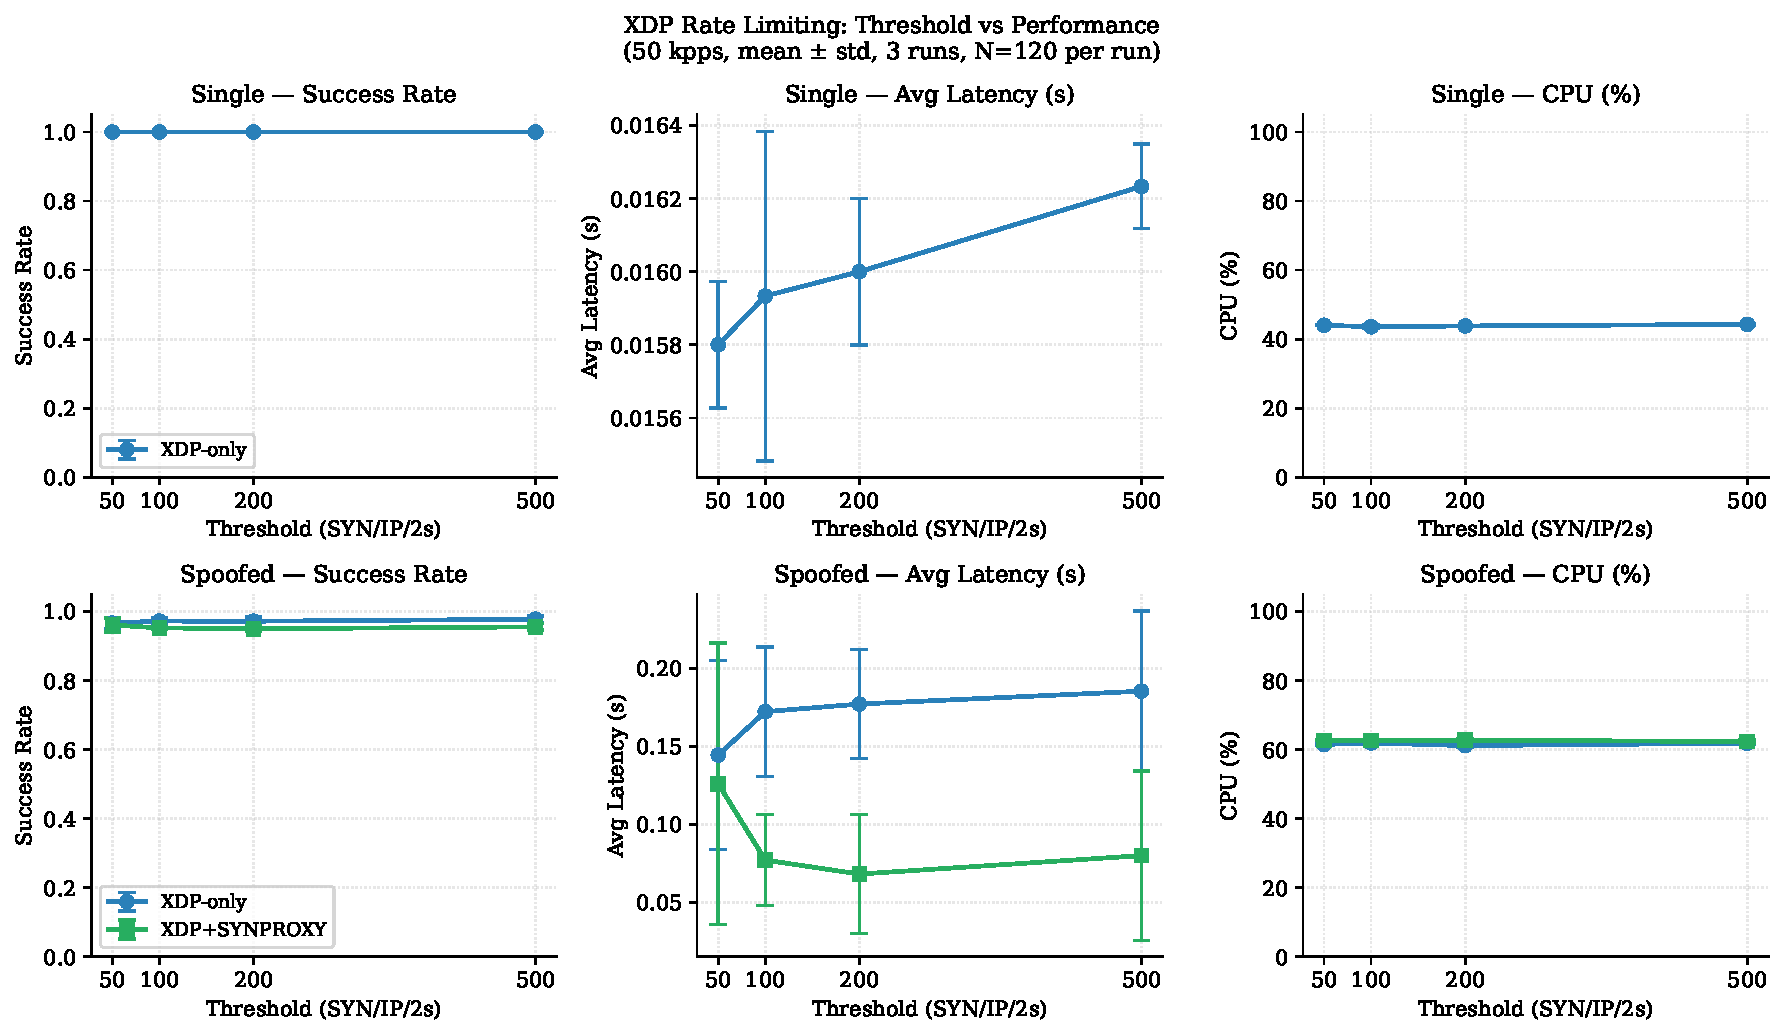
\includegraphics[width=0.48\textwidth]{fig_threshold.pdf}
\caption{Effect of XDP rate limiting threshold $\tau$ on success rate
and latency under single-source and spoofed attacks
(50\,kpps, mean$\pm$std, 3 runs, $N$=120/run).}
\label{fig:threshold}
\end{figure}

% ─────────────────────────────────────────────────────────────────────────────
\subsection{Visualization of Results}

\begin{figure}[h]
\centering

\includegraphics[width=0.48\textwidth]{fig_success_rate.pdf}
\caption{Success rate across configurations and attack scenarios
(emulated testbed, 50\,kpps, mean~$\pm$~std, 3 runs).}
\label{fig:success_rate}
\end{figure}

Figure~\ref{fig:success_rate} shows that all configurations achieve
perfect success under single-source attacks.
Under distributed attacks, XDP+SYNPROXY achieves the best success rate
while iptables+SYNPROXY shows the lowest.
Under spoofed attacks, differences are moderate across all configurations.

\begin{figure}[h]
\centering

\includegraphics[width=0.48\textwidth]{fig_latency.pdf}
\caption{Average latency across configurations and attack scenarios
(emulated testbed, 50\,kpps, mean~$\pm$~std, 3 runs).}
\label{fig:latency}
\end{figure}

Figure~\ref{fig:latency} shows the latency inversion between XDP-only
and iptables+SYNPROXY under spoofed attacks, and the clear latency
advantage of XDP+SYNPROXY under distributed attacks.

\begin{figure}[h]
\centering

\includegraphics[width=0.48\textwidth]{fig_cpu.pdf}
\caption{CPU utilization across configurations and attack scenarios
(emulated testbed, 50\,kpps, mean~$\pm$~std, 3 runs).}
\label{fig:cpu}
\end{figure}

Figure~\ref{fig:cpu} confirms that iptables+SYNPROXY reaches
near-saturation CPU under distributed attacks ($96.7$\%), while
XDP-based configurations maintain consistent efficiency
($43.8$--$62.8$\%) across all scenarios.

% ─────────────────────────────────────────────────────────────────────────────
\section{Conclusion and Future Work}
\label{sec:conclusion}

This paper presented an integrated XDP+SYNPROXY firewall framework for
mitigating SYN flood DDoS attacks, evaluated on both a physical testbed
and a statistically rigorous Mininet-based emulated environment
(3~independent runs, $N=120$ measurements per configuration).

\subsection{Key Contributions and Findings}

\begin{itemize}

  \item \textbf{Scenario-Dependent Effectiveness}:
  No single defense mechanism dominates across all attack scenarios.
  Under single-source attacks, XDP-only provides the best CPU efficiency
  ($43.8 \pm 0.5$\%), a $35$\% reduction over iptables+SYNPROXY.
  Under distributed attacks, XDP+SYNPROXY provides the best latency
  ($0.038 \pm 0.039$\,s) and CPU ($58.3 \pm 0.8$\%).
  Under spoofed attacks, iptables+SYNPROXY provides the lowest latency
  ($0.049 \pm 0.022$\,s).

  \item \textbf{Latency Inversion Under Spoofing}:
  iptables+SYNPROXY achieves lower latency than XDP-only under spoofed
  attacks ($0.049$\,s vs.\ $0.143$\,s, $|d|=5.30$, large effect).
  Connection-level validation prevents spoofed connections from consuming
  server TCP state, reducing backlog pressure more effectively than per-IP
  rate limiting against random source IPs.

  \item \textbf{CPU Saturation Under Distributed Load}:
  iptables+SYNPROXY alone reaches $96.7 \pm 0.6$\% CPU under distributed
  attacks, matching the unprotected baseline ($98.2 \pm 0.4$\%).
  XDP pre-filtering is essential to prevent connection tracking saturation.

  \item \textbf{Optimal Threshold Identification}:
  The threshold sensitivity analysis identifies $\tau=200$~SYN/IP per 2\,s
  as the optimal operating point for XDP+SYNPROXY, achieving the lowest
  latency ($0.068$\,s) under spoofed attacks.
  The runtime-configurable threshold via BPF map enables adaptive
  deployment without program reload.

  \item \textbf{Statistical Validity and Reproducibility}:
  All emulated results are supported by 3~independent runs with $N=120$
  measurements each.
  The very low standard deviations (typically ${<}0.02$ for success rate,
  ${<}1$\% for CPU) and large Cohen's $d$ effect sizes confirm the
  reproducibility and practical significance of the observed differences.

\end{itemize}

\subsection{Limitations and Future Directions}

\begin{itemize}

  \item \textbf{Stateless vs.\ Stateful Coordination}:
  The interaction between XDP and SYNPROXY is indirect.
  Future work should investigate tighter integration via BPF state
  sharing~\cite{bpf_sk_assign_tcp_reqsk}.

  \item \textbf{Performance Under Extreme Load}:
  Future work could explore SmartNIC-based XDP offloading to reduce CPU
  impact~\cite{XDPmode}.

  \item \textbf{Adaptive Threshold Policies}:
  The current implementation uses a static threshold.
  Machine learning-based adaptive policies could dynamically adjust $\tau$
  based on observed traffic patterns, leveraging the runtime configurability
  of the BPF map~\cite{CNN_ddos,dimolianis2022,sidoretti2023}.

  \item \textbf{nftables Integration}:
  As \texttt{nftables} progressively replaces \texttt{iptables} in modern
  Linux distributions, future work should evaluate XDP+nftables-SYNPROXY
  to assess migration paths and performance differences.

  \item \textbf{Formal Statistical Testing}:
  Future work with larger sample sizes ($n \geq 10$) should include
  hypothesis testing (e.g., Wilcoxon signed-rank test) to formally
  characterize the statistical significance of the observed differences.

\end{itemize}

\subsection{Concluding Remarks}

This work demonstrates that combining XDP-based early filtering with
SYNPROXY validation provides a flexible and robust foundation for DDoS
mitigation.
Rather than a one-size-fits-all solution, our findings highlight the
importance of selecting or combining defense mechanisms based on the
attack model.
XDP excels at CPU efficiency and latency under volumetric single-source
attacks; iptables+SYNPROXY excels at latency under spoofed traffic;
XDP+SYNPROXY provides the best balance under distributed attacks.
The runtime-configurable threshold further enables adaptive deployment
without service interruption.

These results contribute to a more nuanced understanding of modern DDoS
defenses and provide practical guidance for deploying XDP and SYNPROXY
in real-world systems~\cite{NetfilterArch,LinuxKernelDoc}.
The source code, experimental artifacts, and datasets are available
at~\cite{GitHubRepo}.

\bibliographystyle{ieeetr}
\bibliography{references}

\end{document}
